%%
%% This is file `pdf-ex.tex',
%% generated with the docstrip utility.
%%
%% The original source files were:
%%
%% pdfpages.dtx  (with options: `example1')
%% 
%% This file demonstrates how to use the pdfpages package.
%%
%% Please send error reports and suggestions for improvements to
%%   Andreas MATTHIAS <andreas.matthias@gmail.com>.
%%
\documentclass[a4paper,12pt]{article}
\usepackage[final]{pdfpages}
\usepackage{verbatim}
%% Uncomment the following lines, if you want to produce thumbnails.
%%\usepackage{pdflscape}
%%\usepackage{thumbpdf}

\newcounter{example}
\setcounter{example}{1}

\newenvironment{example}
  {\par\vskip\topsep%
   \noindent\textbf{Example \arabic{example}:}%
   \stepcounter{example}%
   \par\vskip\topsep%
   \minipage{.9\linewidth}%
   \verbatim}
  {\endverbatim%
   \endminipage\par\vskip\topsep}

\begin{document}

\title{A Demonstration of the \texttt{pdfpages} Package}
\author{Andreas MATTHIAS}
\maketitle

This is a demonstration of the \texttt{pdfpages} package.
It is \textit{not} the documentation of the package.
To get the documentation run: `latex pdfpages.dtx'

\tableofcontents

\section{Inserting Pages:}
\begin{example}

\includepdf[pages=3-5]{dummy.pdf}
\end{example}

\includepdf[pages=3-5]{dummy.pdf}

\section{Using the \texttt{nup} Option}
Arranging several logical pages on one sheet of paper.

\begin{example}

\includepdf[nup=1x2, landscape, pages=4-7]{dummy.pdf}
\end{example}

\includepdf[nup=1x2, landscape, pages=4-7]{dummy.pdf}

Use the option \texttt{turn=false}, if the pages
should not be displayed in landscape orientation.
(If the last two pages were not displayed in
landscape orientation, you use a PDF viewer that
does not support this option.)

\begin{example}

\includepdf[nup=1x2, landscape,
            pages=4-7, turn=false]{dummy.pdf}
\end{example}

\includepdf[nup=1x2, landscape,
            pages=4-7, turn=false]{dummy.pdf}

\begin{example}
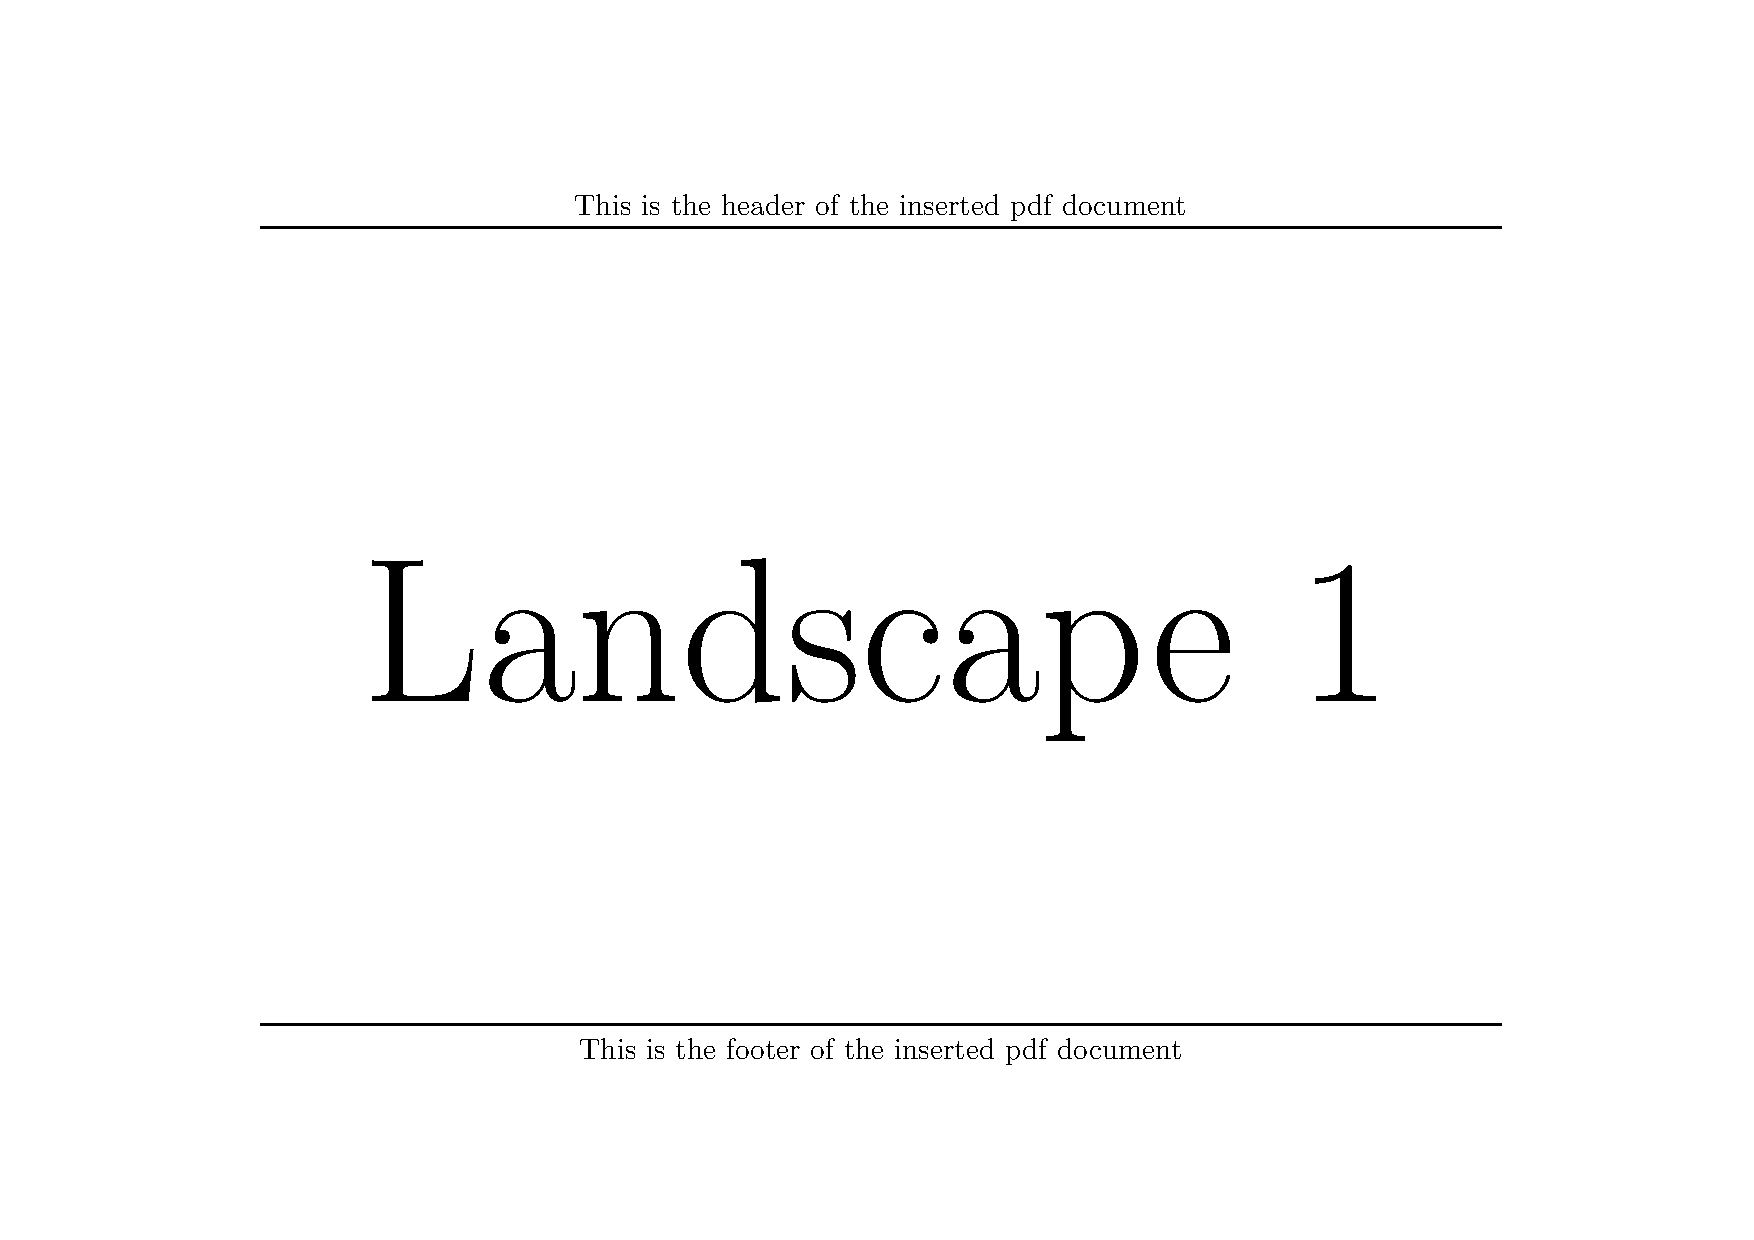
\includepdf[nup=1x2, pages=1-4]{dummy-l.pdf}
\end{example}
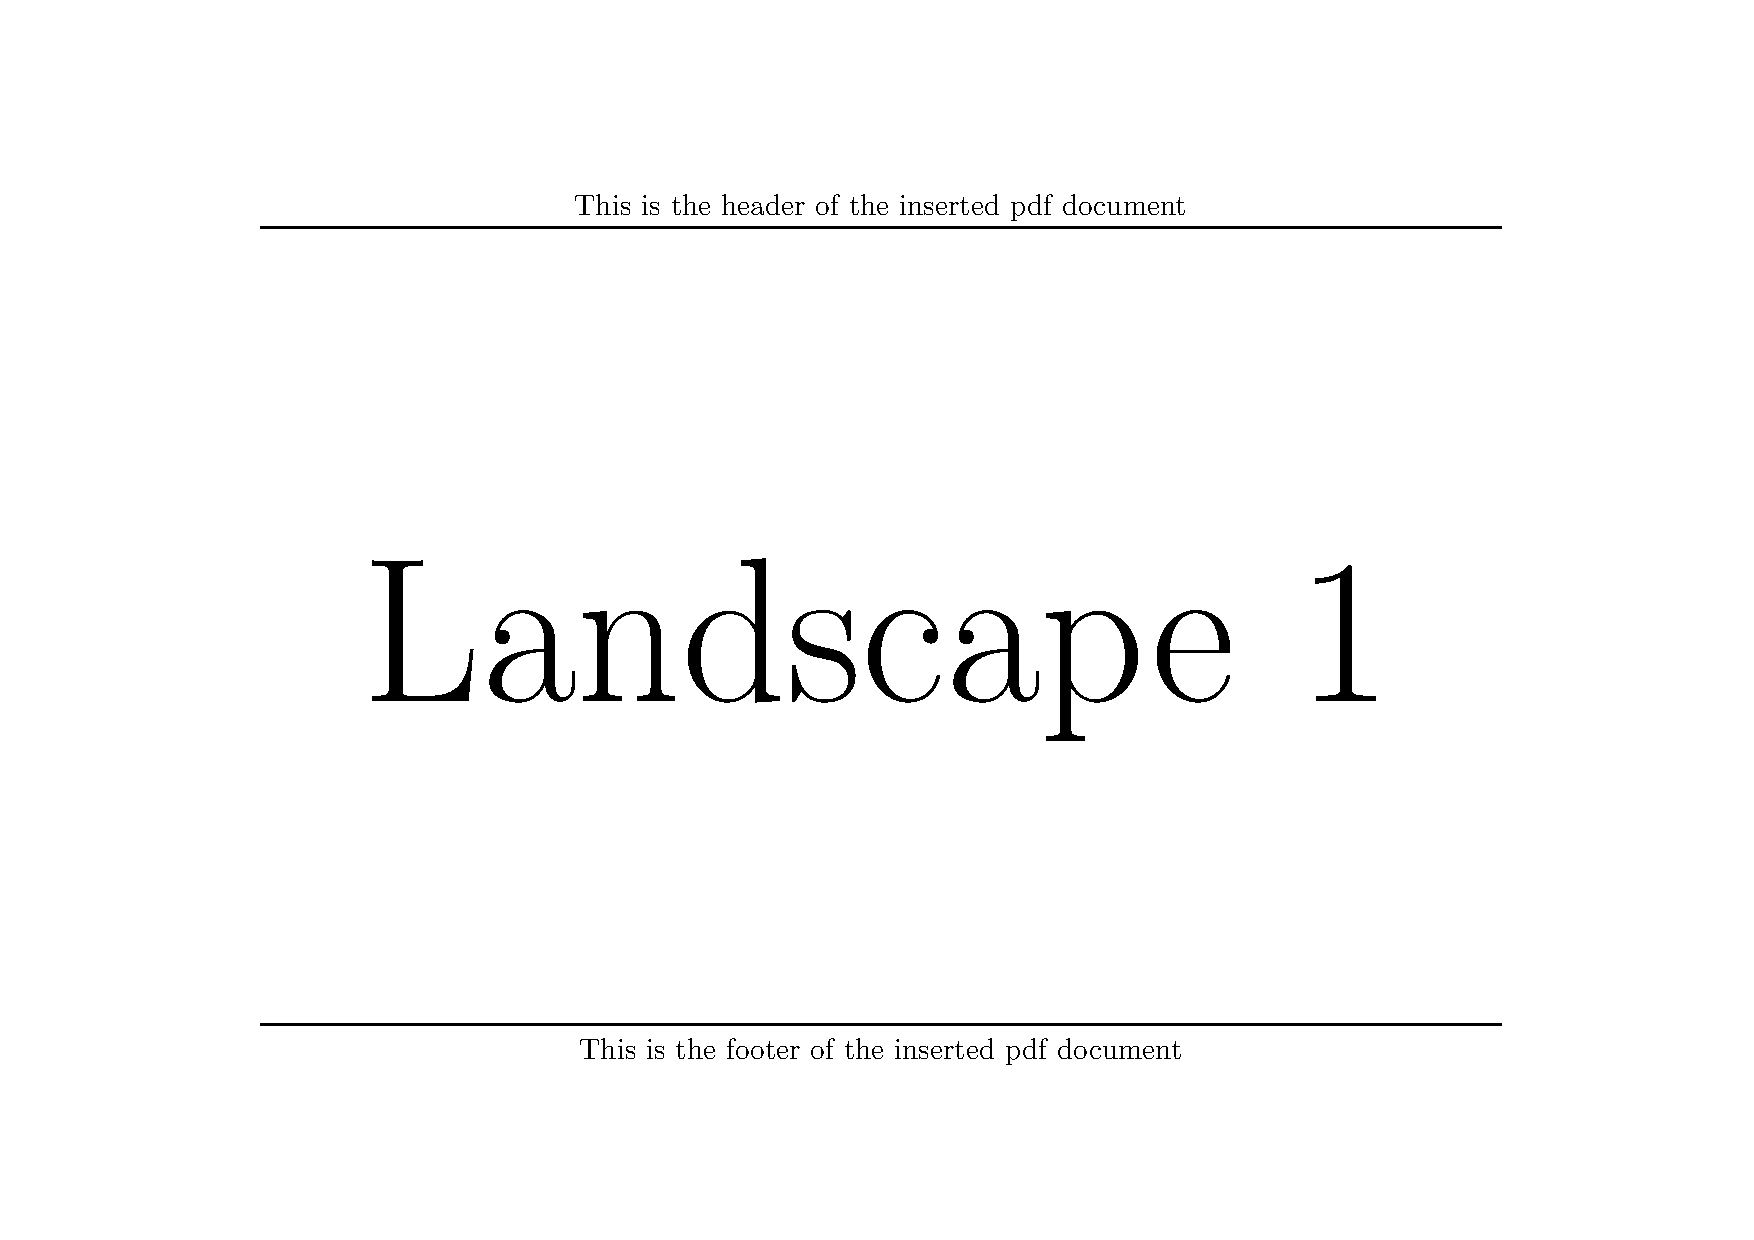
\includepdf[nup=1x2, pages=1-4]{dummy-l.pdf}

\noindent
With the option \texttt{pages} special pages and
ranges of pages can be selected.

\begin{example}

\includepdf[nup=3x2, pages={1,4-6,8,10}]{dummy.pdf}
\end{example}

\includepdf[nup=3x2, pages={1,4-6,8,10}]{dummy.pdf}

\noindent
A column-major layout can be achieved with the
option \texttt{column}.

\begin{example}

\includepdf[nup=2x2, pages=1-4, column]{dummy.pdf}
\end{example}

\includepdf[nup=2x2, pages=1-4, column]{dummy.pdf}

\noindent
Sometimes it might be useful to put an empty page
at the beginning.
\begin{example}

\includepdf[nup=2x2, pages={{},5-7}]{dummy.pdf}
\end{example}

\includepdf[nup=2x2, pages={{},5-7}]{dummy.pdf}

\section{Changing Layout}

To put some space between the logical pages, use the option
\texttt{delta}.

Any options of \verb|\includegraphics| are allowed in
\verb|\includepdf| as well. See the \texttt{scale}
option in the next example.
\begin{example}

\includepdf[nup=2x2, pages=3-6, scale=.8,
            delta=8mm 11mm, frame]{dummy.pdf}
\end{example}

\includepdf[nup=2x2, pages=3-6, scale=.8,
            delta=8mm 11mm, frame]{dummy.pdf}

\noindent
By default the output is centered, as you could see in
the last examples. With the \texttt{offset} option it is
possible to displace the output.

\begin{example}

\includepdf[nup=2x2, pages=3-6, scale=.8,
            offset=5mm 7mm, frame]{dummy.pdf}
\end{example}

\includepdf[nup=2x2, pages=3-6, scale=.8,
            offset=5mm 7mm, frame]{dummy.pdf}

\noindent
To remove the header and the footer of the inserted
document use the \texttt{trim} and \texttt{clip}
options of the \texttt{graphicx} package.

\begin{example}

\includepdf[nup=2x2, pages=1-4,
            trim=0 40mm 0 40mm,
            clip, pagecommand={}]{dummy.pdf}
\end{example}

\noindent The option
\verb|pagecommand={\thispagestyle{empty}}|
is set by default. If you don't want the page style
to be set to empty, you can remove this default
setting by using the \texttt{pagecommand} option
as follows:
\verb|pagecommand={}|.


\includepdf[nup=2x2, pages=1-4,
            trim=0 40mm 0 40mm,
            clip, pagecommand={}]{dummy.pdf}

\noindent
You like the crazy way? Then try this one \texttt{;-)}
\begin{example}

\includepdf[pages={3,4}, nup=1x2,
            landscape, scale=1.1,
            angle=30, delta=0 -85mm]{dummy.pdf}
\end{example}

\includepdf[pages={3,4}, nup=1x2,
            landscape, scale=1.1,
            angle=30, delta=0 -85mm]{dummy.pdf}

\end{document}
\endinput
%%
%% End of file `pdf-ex.tex'.
